\documentclass{article}

\usepackage[utf8]{inputenc}
\usepackage[brazil]{babel}
\usepackage{longtable}
\usepackage{graphicx}
\usepackage{hyperref}
\usepackage[top=2cm, bottom=2cm, left=2cm, right=2cm]{geometry}

\title{Caixeiro Viajante com ACO}
\author{Vinícius Couto Tasso}

\begin{document}
\maketitle

A atividade proposta traz uma instância do clássico \textit{Travelling Salesman Problem} (TSP) utilizando \textit{Ant Colony Optimization}. Os dados utilizados são constituídos por uma lista com as coordenadas geográficas de 5851 cidades diferentes, sendo a maioria delas cidades brasileiras.

Foi utilizado o software ACOTSP\footnote{Disponível em \url{http://iridia.ulb.ac.be/~mdorigo/ACO/aco-code/public-software.html}}, específico para a aplicação de ACO para problemas TSP. Conforme sugerido pelo enunciado do problema, foram utilizadas variações dos valores de parâmetro \textit{default} ($\alpha=1.0$, $\beta=2.0$ e $\rho=0.5$) de -50\% até +100\%. Cada parâmetro assumiu 4 valores diferentes dentro de seus respectivos intervalos, resultando em 64 combinações diferentes testadas.

Para cada combinação de parâmetros, foi realizada uma bateria de 10 experimentos, cada um com uma nova semente aleatória. Foram utilizadas a média entre o melhor resultado de cada rodada, bem como o melhor resultado entre todas. A relação de parâmetros utilizados e resultados obtidos pode ser vista na Tabela \ref{tab:res}.

A Figura \ref{fig:beta} apresenta a relação entre o melhor resultado obtido (eixo y), o valor do parâmetro $\alpha$ (eixo x) e o valor de $\beta$ (cor dos pontos). Similarmente, a Figura \ref{fig:rho} traz os mesmos valores nos eixos x e y, mas a cor dos pontos é definida pelo valor de $\rho$.

\begin{figure}[htbp!]
  \centering
  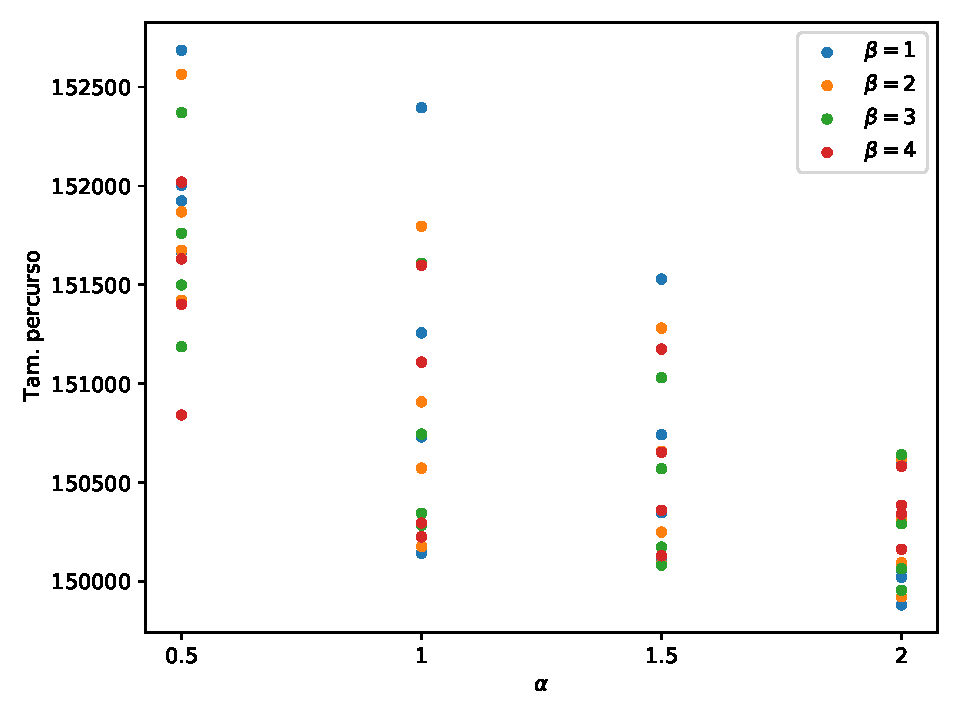
\includegraphics[scale=0.8]{beta.pdf}
  \caption{Tamanho do percurso mínimo por $\alpha$ e $\beta$}
  \label{fig:beta}
\end{figure}

Podemos observar que os resultados tem uma tendência a melhorar (diminuir) conforme o valor de $\alpha$ (influência dos feromônios) aumenta. Isso pode ser um indicador de que, para valores muito baixos, os caminhos promissores (que continham feromônio) não eram bem explorados, dificultando um eventual ajuste fino em soluções encontradas. Entretanto, aumentar muito este valor fará com que a busca seja muito localizada, fazendo com que o algoritmo seja propício a convergir rapidamente para mínimos locais.

Para diferentes valores de $\beta$, a tendência é um pouco diferente: não parece haver uma separação muito clara entre os resultados para os diferentes valores do parâmetro, havendo uma variação aparentemente baixa. Isso sugere que a influência da busca aleatória, determinada por este parâmetro, já é alta o suficiente para explorar caminhos diferentes mesmo quando o parâmetro assuem o menor valor utilizado.

\begin{figure}[htbp!]
  \centering
  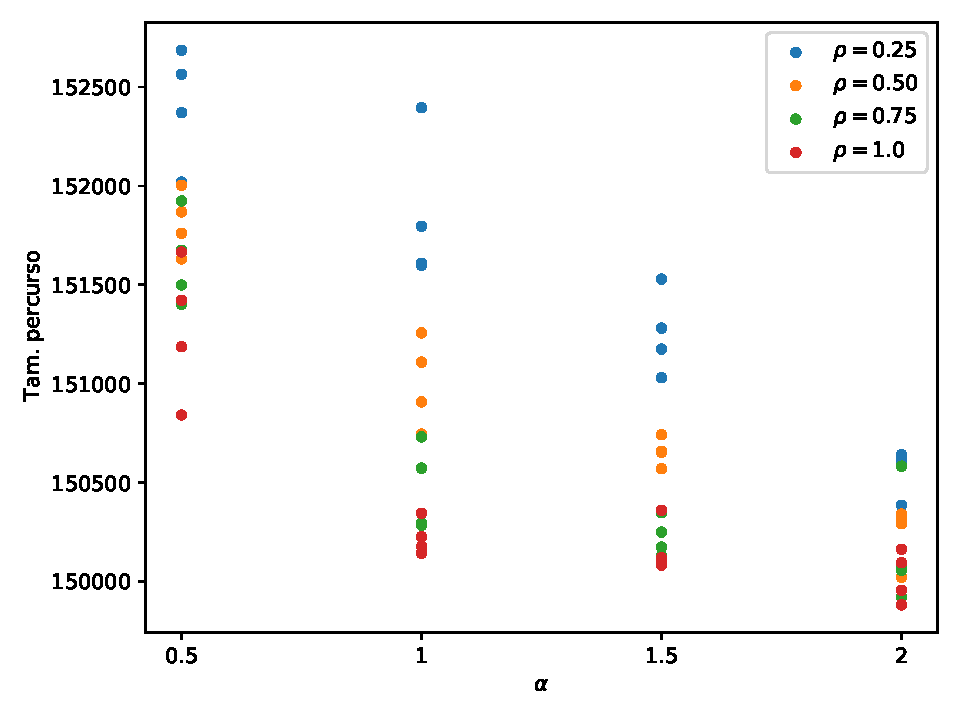
\includegraphics[scale=0.8]{rho.pdf}
  \caption{Tamanho do percurso mínimo por $\alpha$ e $\rho$}
  \label{fig:rho}
\end{figure}

Por fim, existe a influência da evaporação das trilhas de feromônio, determinada pelo parâmetro $\rho$. Aqui podemos ver uma separação mais clara, principalmente para $\alpha = 1$ e $\alpha = 1.5$, entre valores baixos ($\rho \leq 0.5$) e altos ($\rho \geq 0.5$). Aparentemente, para valores mais baixos, o tempo de evaporação das trilhas é muito baixo, o que pode prejudicar a integridade de um caminho que já foi descoberto, impedindo que seja devidamente explorado.

Mais detalhes sobre os experimentos realizados podem ser encontrados na tabela a seguir.

  \begin{longtable}[htbp]{|c|c|c|c|c|}
    \hline
    \textbf{Alpha} $(\alpha)$ & \textbf{Beta} $(\beta)$ & \textbf{Rho} $(\rho)$ & \textbf{Média} &  \textbf{Melhor resultado} \\ \hline

    0.5 & 1 & 0.25 & 153268 & 152686 \\ \hline
    0.5 & 1 & 0.50 & 152944 & 152003 \\ \hline
    0.5 & 1 & 0.75 & 152565 & 151924 \\ \hline
    0.5 & 1 & 1.00 & 152226 & 151666 \\ \hline
    0.5 & 2 & 0.25 & 153137 & 152564 \\ \hline
    0.5 & 2 & 0.50 & 152671 & 151869 \\ \hline
    0.5 & 2 & 0.75 & 152296 & 151674 \\ \hline
    0.5 & 2 & 1.00 & 151915 & 151422 \\ \hline
    0.5 & 3 & 0.25 & 153019 & 152371 \\ \hline
    0.5 & 3 & 0.50 & 152489 & 151760 \\ \hline
    0.5 & 3 & 0.75 & 152074 & 151499 \\ \hline
    0.5 & 3 & 1.00 & 151758 & 151187 \\ \hline
    0.5 & 4 & 0.25 & 152848 & 152019 \\ \hline
    0.5 & 4 & 0.50 & 152302 & 151631 \\ \hline
    0.5 & 4 & 0.75 & 151981 & 151401 \\ \hline
    0.5 & 4 & 1.00 & 151589 & 150842 \\ \hline
    1.0 & 1 & 0.25 & 152931 & 152396 \\ \hline
    1.0 & 1 & 0.50 & 152076 & 151257 \\ \hline
    1.0 & 1 & 0.75 & 151350 & 150731 \\ \hline
    1.0 & 1 & 1.00 & 150858 & 150142 \\ \hline
    1.0 & 2 & 0.25 & 152577 & 151796 \\ \hline
    1.0 & 2 & 0.50 & 151850 & 150908 \\ \hline
    1.0 & 2 & 0.75 & 151186 & 150573 \\ \hline
    1.0 & 2 & 1.00 & 150888 & 150177 \\ \hline
    1.0 & 3 & 0.25 & 152348 & 151608 \\ \hline
    1.0 & 3 & 0.50 & 151679 & 150745 \\ \hline
    1.0 & 3 & 0.75 & 151154 & 150285 \\ \hline
    1.0 & 3 & 1.00 & 150905 & 150345 \\ \hline
    1.0 & 4 & 0.25 & 152217 & 151598 \\ \hline
    1.0 & 4 & 0.50 & 151647 & 151109 \\ \hline
    1.0 & 4 & 0.75 & 151111 & 150296 \\ \hline
    1.0 & 4 & 1.00 & 150882 & 150226 \\ \hline
    1.5 & 1 & 0.25 & 152225 & 151529 \\ \hline
    1.5 & 1 & 0.50 & 151454 & 150742 \\ \hline
    1.5 & 1 & 0.75 & 150877 & 150348 \\ \hline
    1.5 & 1 & 1.00 & 150749 & 150120 \\ \hline
    1.5 & 2 & 0.25 & 151940 & 151281 \\ \hline
    1.5 & 2 & 0.50 & 151310 & 150658 \\ \hline
    1.5 & 2 & 0.75 & 150796 & 150250 \\ \hline
    1.5 & 2 & 1.00 & 150761 & 150088 \\ \hline
    1.5 & 3 & 0.25 & 151828 & 151030 \\ \hline
    1.5 & 3 & 0.50 & 151222 & 150570 \\ \hline
    1.5 & 3 & 0.75 & 150748 & 150174 \\ \hline
    1.5 & 3 & 1.00 & 150859 & 150083 \\ \hline
    1.5 & 4 & 0.25 & 151722 & 151175 \\ \hline
    1.5 & 4 & 0.50 & 151214 & 150653 \\ \hline
    1.5 & 4 & 0.75 & 150715 & 150130 \\ \hline
    1.5 & 4 & 1.00 & 150912 & 150360 \\ \hline
    2.0 & 1 & 0.25 & 151528 & 150613 \\ \hline
    2.0 & 1 & 0.50 & 151000 & 150022 \\ \hline
    2.0 & 1 & 0.75 & 150663 & 150057 \\ \hline
    2.0 & 1 & 1.00 & 150603 & 149882 \\ \hline
    2.0 & 2 & 0.25 & 151391 & 150619 \\ \hline
    2.0 & 2 & 0.50 & 150898 & 150317 \\ \hline
    2.0 & 2 & 0.75 & 150620 & 149924 \\ \hline
    2.0 & 2 & 1.00 & 150731 & 150095 \\ \hline
    2.0 & 3 & 0.25 & 151309 & 150642 \\ \hline
    2.0 & 3 & 0.50 & 150885 & 150292 \\ \hline
    2.0 & 3 & 0.75 & 150612 & 150065 \\ \hline
    2.0 & 3 & 1.00 & 150798 & 149955 \\ \hline
    2.0 & 4 & 0.25 & 151306 & 150385 \\ \hline
    2.0 & 4 & 0.50 & 150858 & 150341 \\ \hline
    2.0 & 4 & 0.75 & \textbf{150583} & \textbf{149865} \\ \hline
    2.0 & 4 & 1.00 & 150787 & 150163 \\ \hline

    \caption{Relação de parâmetros utilizados e resultados obtidos}
    \label{tab:res}
  \end{longtable}

\end{document}
